\documentclass{article}

\pdfoutput=1
\usepackage{mathtools}
\usepackage{amsmath}
\usepackage{amsfonts}
\usepackage{amssymb}
\usepackage{graphicx}
\usepackage{epsfig}
\usepackage{color}
\usepackage{float}
\usepackage{hyperref}
\usepackage{verbatim}
\usepackage{fancyhdr} 
\usepackage{amsthm}
\usepackage{bbold}
\usepackage{verbatim}
\usepackage{slashed}
\usepackage{setspace}
\usepackage{listings}
\usepackage{pgfplots}
\pgfplotsset{compat = newest}
\hypersetup{
    colorlinks=true,
    linkcolor=blue,
    filecolor=magenta,      
    urlcolor=blue,
}

\begin{document}

\title{CS146 Assignment 1 Diagnostic Problem Set}

\section{Discrete probabilities}

Exercise 6.1 from Deisenroth, M.P, Faisal, A.A., Ong, C.S., (2020). \href{https://mml-book.github.io/book/mml-book.pdf}{Mathematics for Machine Learning}. Cambridge University Press.

Consider the following joint distribution, $p(x, y)$, over two discrete random variables $X$ and $Y$ .
    
\begin{center}
    \begin{tabular}{ |c|c|c|c|c|c| } 
        \hline
        $y_{1}$ & 0.01 & 0.02 & 0.03 & 0.1 & 0.1 \\ 
        \hline
        $y_{2}$ & 0.05 & 0.1 & 0.05 & 0.07 & 0.2 \\
        \hline 
        $y_{3}$ & 0.1 & 0.05 & 0.03 & 0.05 & 0.04 \\ 
        \hline
         & $x_{1}$ & $x_{2}$ & $x_{3}$ & $x_{4}$ & $x_{5}$ \\ 
        \hline
    \end{tabular}
\end{center}

\begin{enumerate}
    \item Compute the marginal distributions $p(x)$ and $p(y)$.
    
    For $p(x)$, we sum the columns.
        \begin{center}
            \begin{tabular}{ |c|c|c|c|c| } 
                \hline
                $x_{1}$ & $x_{2}$ & $x_{3}$ & $x_{4}$ & $x_{5}$ \\ 
                \hline
                0.16 & 0.17 & 0.11 & 0.22 & 0.34 \\
                \hline
            \end{tabular}
        \end{center}

    For $p(y)$ we sum the rows.
        \begin{center}
            \begin{tabular}{ |c|c| } 
                \hline
                $y_{1}$ & 0.26 \\ 
                \hline
                $y_{2}$ & 0.47 \\
                \hline 
                $y_{3}$ & 0.27 \\
                \hline
            \end{tabular}
        \end{center}
    \item Compute the conditional distribution $p(x | Y = y_{1})$.
    
    For the conditional probability we take the joint probability, $p(x = x, y = y_{1})$ , divided by the marginal probability, $p(y = y_{1})$.
        \begin{center}
            \begin{tabular}{ |c|c|c|c|c|c| } 
                \hline
                $y_{1}$ & 0.03846153846 & 0.07692307692 & 0.1153846154 & 0.3846153846 & 0.3846153846 \\  
                \hline
                & $x_{1}$ & $x_{2}$ & $x_{3}$ & $x_{4}$ & $x_{5}$ \\ 
                \hline
            \end{tabular}
        \end{center}
    \item Compute the conditional distribution $p(y | X = x_{3})$.
    
    For the conditional probability we take the joint probability, $p(x = x_{3}, y = y)$ , divided by the marginal probability, $p(x = x_{3})$.
        \begin{center}
            \begin{tabular}{ |c|c| } 
                \hline
                $y_{1}$ & 0.2727272727 \\ 
                \hline
                $y_{2}$ & 0.4545454545 \\
                \hline 
                $y_{3}$ & 0.2727272727 \\ 
                \hline
                & $x_{3}$ \\ 
                \hline
            \end{tabular}
        \end{center}
\end{enumerate}

\section{Calculating probabilities}

\begin{enumerate}
    \item How many students are in your CS146 class, including yourself? (Take a guess if you’re not entirely sure.)
        
    There are 18 students. That means 17 other classmates (excluding myself).

    \item Assuming you know nothing about your classmates —
            \begin{enumerate}
                \item What is the probability that you were born after all of them?
                
                Given that I know nothing about the classmates, and dates are continuos (before big bang - future), we can 
                start with the following probabilities. If I pick a person, there is 1/3 chance they were born before me,
                1/3 chance we were born on the same day and 1/3 chance they were born after me. Therefore, the probability that
                I was born after all of my classmates, it is the probability that they were all born before me.

                $$\left(\frac{1}{3}\right)^{17} = 0.000000007743524$$

                \item What is the probability that you were born before all of them?
                
                As we mentioned above given that the probability I was born before a single person is 1/3, then
                the probability of being born before all the 17 classmates is (similar to a):

                $$\left(\frac{1}{3}\right)^{17} = 0.000000007743524$$

                \item What is the probability that you were born after at least half of the other students?
                
                The probability I was born after is 1/3 and the probability of not being born after is 2/3. This would
                require us to use a binomial distribution. 

                Half the number of students is 17/2 = 8.5. Let us use the lower bound 8 and the upper bound 9 to provide
                2 answers.

                The probability of being born after at least 8 students is the summation of the probabilities of being born
                after 1 student, 2 students, ..., 8 students.

                $$^{n}C_{x} p^{x} (1 - p)^{n-x}$$

                $$^{n}C_{x} = \frac{n!}{x!(n-x)!}$$

                Given that $n = 17$, $x = 1$, $p = \frac{1}{3}$:

                $$p(x = 1) = \frac{17!}{1!(17-1)!} \left(\frac{1}{3}\right)^{1} \left(1 - \frac{1}{3}\right)^{17-1} = 0.008627153428635511$$

                $$p(x = 2) = \frac{17!}{2!(17-2)!} \left(\frac{1}{3}\right)^{2} \left(1 - \frac{1}{3}\right)^{17-2} = 0.03450861371454206$$

                $$p(x = 3) = \frac{17!}{3!(17-3)!} \left(\frac{1}{3}\right)^{3} \left(1 - \frac{1}{3}\right)^{17-3} = 0.08627153428635512$$

                $$p(x = 4) = \frac{17!}{4!(17-4)!} \left(\frac{1}{3}\right)^{4} \left(1 - \frac{1}{3}\right)^{17-4} = 0.15097518500112148$$

                $$p(x = 5) = \frac{17!}{5!(17-5)!} \left(\frac{1}{3}\right)^{5} \left(1 - \frac{1}{3}\right)^{17-5} = 0.1962677405014579$$

                $$p(x = 6) = \frac{17!}{6!(17-6)!} \left(\frac{1}{3}\right)^{6} \left(1 - \frac{1}{3}\right)^{17-6} = 0.1962677405014579$$

                $$p(x = 7) = \frac{17!}{7!(17-7)!} \left(\frac{1}{3}\right)^{7} \left(1 - \frac{1}{3}\right)^{17-7} = 0.1542103675368598$$

                $$p(x = 8) = \frac{17!}{8!(17-8)!} \left(\frac{1}{3}\right)^{8} \left(1 - \frac{1}{3}\right)^{17-8} = 0.09638147971053737$$

                $$p(x = 9) = \frac{17!}{9!(17-9)!} \left(\frac{1}{3}\right)^{9} \left(1 - \frac{1}{3}\right)^{17-9} = 0.048190739855268686$$

                Therefore, after doing the lower bound is $0.9245247739078654$, while the upper bound is $0.972715513763134$.

            \end{enumerate}
\end{enumerate}

\section{Normal distribution}

If $x$ is distributed according to the \href{https://en.wikipedia.org/wiki/Normal_distribution}{normal distribution} with mean $\mu$ and standard deviation $\sigma$ , and
if $f(x)=x^{3} +2x+1$.

\begin{enumerate}
    \item Calculate the expected value of $f (x)$.

    Given that $x$ is from a normal distribution, it's expected value is $0$. Therefore, plugging that into the equation produces:
    $0^{3} + 2 \times 0 + 1 = 1$.

    To make it more general, the expected value of a normal distribution is $\mu$, therefore, if we plug that into the equation, then, we
    get the expected value for $f(x)$. 
    $$f(\mu) = \mu^{3} + 2 \mu + 1$$
    \item Calculate the probability $P ( f (x) > 1 )$.
    
    Values that generate $f(x) > 1$ are $[0, \infty)$

    \begin{center}
        \begin{tikzpicture}
            \begin{axis}[
                xmin = -5, xmax = 5,
                ymin = -1, ymax = 3]
                \addplot[
                    samples = 100
                ]{x^3 + 2*x + 1};
            \end{axis}
        \end{tikzpicture}
    \end{center}

    Therefore, we only need to find the probability of getting an $x$ value greater than $0$.

    \begin{figure}[H]
        \centering
        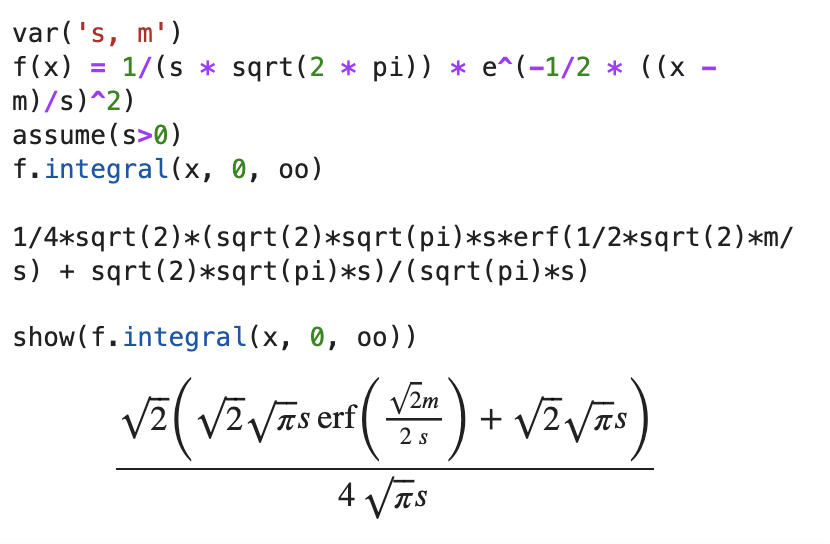
\includegraphics[width=300 pt]{problem.png}
        \label{fig:my_label}
        \caption{Sage math computation for the integral of a normal distribution from}
    \end{figure} 

    \item Write a Python script to confirm your answer to question 2. Generate a lot of random numbers from a normal distribution with a particular mean and standard deviation. Calculate $f (x)$ for each of these random numbers. How many of them are greater than 1? Does that match the probability you calculated in question 2?
    
    \begin{figure}[H]
        \centering
        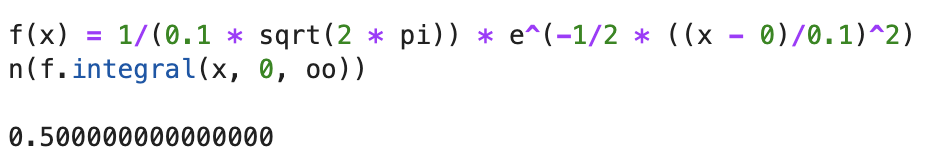
\includegraphics[width=300 pt]{solution.png}
        \label{fig:my_label}
        \caption{Example probability}
    \end{figure} 

    \begin{lstlisting}[language=Python]
    import numpy as np

    mu, sigma = 0, 0.1  # mean and standard deviation

    s = np.random.normal(mu, sigma, 1000)

    y = np.array(
        list(map(lambda x: x**3 + 2*x + 1, s))
    )

    sum(y > 1)
    \end{lstlisting}

    The answer was 505, which means 505/1000 was the probability.


\end{enumerate}

\section{Double-headed coin}

Adapted from exercise 2.6 from Blitzstein, J.K., Hwang, J. (2019). \href{https://drive.google.com/file/d/1VmkAAGOYCTORq1wxSQqy255qLJjTNvBI/view}{Introduction to Probability, 2nd Edition}, Taylor \& Francis Group.

A bag contains 1000 coins, where 999 are normal (they land on heads 50\% of the time) and 1 coin is double-headed (lands on heads 100\% of the time). A coin is chosen uniformly at random and flipped 10 times. It lands on heads every time – so, 10 heads in a row.

\textbf{Question 1} Given this information, what is the probability that the chosen coin is the double-headed coin?

Given that $D = $ double head, $S = $ 10 heads:

$$p(D) = 1/1000$$

$$p(\neg D) = 999/1000$$

$$p(head | D) = 1$$

$$p(head | \neg D) = 0.5$$

$$p(D | S) = \frac{p(S | D) p(D)}{p(S)}$$

$$p(S| D) = p(head | D)^{10} = 1$$

$$p(S) = p(S |D)p(D) + p(S | \neg D)p(\neg D)$$

$$p(S | \neg D) = p(head | \neg D)^{10} = 0.5^{10}$$

$$p(S) = 1 \times 1/1000 + 0.5^{10} \times 999/1000 = 0.001975585938$$

$$p(D | S) = \frac{1 \times 1/1000}{0.001975585938} = 0.506178942$$


\textbf{Question 2} You should find that the answer to Question 1 is approximately $\frac{1}{2}$. I find this surprising. Explain as straightforwardly as you can (without using complicated math) why we should, in fact, expect the result to be approximately $\frac{1}{2}$.

For a normal fair coin, the chance of flipping a head is 0.5. The chance of flipping a second head independently is 0.5 too. However, 
the probability of flipping head twice we have to measure it against all other outcomes (HH, TH, HT, TT). It only occurs once (0.25)[$0.5^{2}$].
Therefore, the more we flip the more options we generate and therefore, the smaller the probability of getting subsequent values.

In our problem when we flip it 10 times and only get heads, the probability is really low for a normal coin, however, for a double headed
coin, the probability is 1 since it is always the outcome. Therefore, the chances of picking a double sided coin and getting 10 heads remains
constant while for picking a normal coin and flipping 10 heads is extremely small (reducing after each flip). That means the more we flip and 
we only get heads, our confidence that we do have the double sided coin will keep increasing since the probability that it is a normal coin
is reducing.

\section{Smokers}

Exercise 2.3 from Blitzstein, J.K., Hwang, J. (2019). \href{https://drive.google.com/file/d/1VmkAAGOYCTORq1wxSQqy255qLJjTNvBI/view}{Introduction to Probability, 2nd Edition}, Taylor \& Francis Group.

According to the CDC (Centers for Disease Control and Prevention) in the USA, men who smoke are 23 times more likely to develop lung cancer than men who don’t smoke. Also according to the CDC, 21.6\% of men in the U.S.A. smoke. What is the probability that a man in the U.S.A. is a smoker, given that he develops lung cancer?

$$p(smoke) = 0.216$$

$$p(\neg smoke) = 1 - p(smoke) = 1 - 0.216 = 0.784$$

$$\frac{p(cancer | smoke)}{p(cancer | \neg smoke)} = 23$$

$$\therefore p(cancer | \neg smoke) = \frac{p(cancer | smoke)}{23}$$

$$p(smoke | cancer) = \frac{p(cancer | smoke) p(smoke)}{p(cancer)}$$

$$p(cancer) = p(cancer|smoke)p(smoke) + p(cancer|\neg smoke)p(\neg smoke)$$

$$p(cancer) = 0.216  \times p(cancer|smoke) + 0.784 \times \frac{p(cancer | smoke)}{23}$$

$$p(cancer) = p(cancer|smoke) \left ( 0.216  + \frac{0.784}{23} \right )$$

$$p(cancer) = p(cancer|smoke) \left ( 0.2500869565 \right )$$

$$p(smoke | cancer) = \frac{p(cancer | smoke) \times 0.216 }{0.2500869565 \times p(cancer|smoke)} = \frac{0.216}{0.2500869565}$$

Therefore, the probability that a person is a smoker given they develop cancer is 0.8636995828. A high value suggesting
smoking may have something to do with cancer causally.

\section*{Appendix}

\subsection*{Code used in problem 2 calculating probabilities}

\begin{lstlisting}[language=Python]
from math import factorial

def comp(n):
    return  (factorial(17))/(
            factorial(n)*factorial(17-n)
        )*(1/3)**n * (2/3)**(17-n)
\end{lstlisting}

\end{document}
